\begin{solution}
\begin{enumerate}
\item {[4 points]} We can compute that, for $n=1,2,\ldots$,
\begin{eqnarray*}
\left(L \psi_n\right)(x) &=& -\psi_n''(x) + \psi_n''''(x)
\\
&=& -{d^2 \over dx^2} (\sqrt{2} \sin(n\pi x)) + {d^4\over dx^4}(\sqrt{2} \sin(n\pi x))
\\
&=& n^2\pi^2 \sqrt{2} \sin(n\pi x) + n^4\pi^4 \sqrt{2}\sin(n\pi x)
\\
&=& (n^2\pi^2 + n^4\pi^4) \psi_n(x).
\end{eqnarray*} 
Hence,
\[
\lambda_n = n^2\pi^2 + n^4\pi^4\mbox{ for }n=1,2,\ldots.
\]
\\
\item {[7 points]} Substituting the expression for $u(x,t)$ into the partial differential equation yields
\[
\sum_{n=1}^\infty a_n'(t) \psi_n(x) = \sum_{n=1}^\infty a_n(t) (\psi_n''(x) - \psi_n''''(x))
\]
and hence
\[
\sum_{n=1}^\infty a_n'(t) \psi_n(x) = \sum_{n=1}^\infty (-\lambda_n) a_n(t) \psi_n(x).
\]
We can then say that
\[
\sum_{n=1}^\infty a_n'(t) \int_0^1\psi_n(x)\psi_m(x)\,dx = \sum_{n=1}^\infty (-\lambda_n) a_n(t) \int_0^1\psi_n(x)\psi_m(x)\,dx,
\]
for $m=1,2,\ldots$, from which it follows that
\[
a_m'(t) = -\lambda_m a_m(t),
\]
for $m=1,2,\ldots$, since
\[
\int_0^1\psi_n(x)\psi_m(x)\,dx=\left\{\begin{array}{rl}1 & \mbox{if }m=n \\ 0 & \mbox{if }m\ne n\end{array}\right.
\]
for $m,n=1,2,\ldots$.

Also,
\[
u(x,0)=u_0(x)
\]
means that
\[
\sum_{n=1}^\infty a_n(0) \psi_n(x)=u_0(x)
\]
and so
\[
\sum_{n=1}^\infty a_n(0) \int_0^1\psi_n(x)\psi_m(x)\,dx=\int_0^1u_0(x)\psi_m(x)\,dx,
\]
for $m=1,2,\ldots$, from which it follows that
\[
a_m(0)=\int_0^1u_0(x)\psi_m(x)\,dx,
\]
for $m=1,2,\ldots$, since
\[
\int_0^1\psi_n(x)\psi_m(x)\,dx=\left\{\begin{array}{rl}1 & \mbox{if }m=n \\ 0 & \mbox{if }m\ne n\end{array}\right.
\]
for $m,n=1,2,\ldots$.

Hence, for $n=1,2,\ldots$, $a_n(t)$ is the solution to the differential equation
\[
a_n'(t) = -\lambda_n a_n(t)
\]
with initial condition
\[
a_n(0)=\int_0^1u_0(x)\psi_n(x)\,dx.
\]

\item {[3 points]} For $n=1,2,\ldots$,
\begin{eqnarray*}
a_n(t)&=&\int_0^1u_0(x)\psi_n(x)\,dx e^{-\lambda_n t}
\\
&=&\int_0^1\sqrt{2}u_0(x)\sin(n\pi x)\,dx e^{-(n^2\pi^2 + n^4\pi^4)t}
\\
&=&b_n e^{-(n^2\pi^2 + n^4\pi^4)t}
\end{eqnarray*}
where
\[
b_n=\left\{ \begin{array}{cl} \displaystyle{{432\sqrt{2} (n^4-18n^2 + 216) \over (36n-n^3)^3 \pi^3}} & \mbox{if }n\mbox{ is odd}; \\0 & \mbox{if }n\mbox{ is even}.\end{array}\right.
\]
\\
\item {[3 points]} We can write
\begin{eqnarray*}
u(x,t) &=& \sum_{n=1}^\infty a_n(t) \psi_n(x)
\\
&=& \sum_{n=1}^\infty b_n e^{-(n^2\pi^2 + n^4\pi^4)t} \psi_n(x)
\\
&=& \sum_{n=1}^\infty c_n e^{-(n^2\pi^2 + n^4\pi^4)t} \sin(n\pi x)
\end{eqnarray*}
where
\[
c_n=\left\{ \begin{array}{cl} \displaystyle{{864 (n^4-18n^2 + 216) \over (36n-n^3)^3 \pi^3}} & \mbox{if }n\mbox{ is odd}; \\0 & \mbox{if }n\mbox{ is even}.\end{array}\right.
\]
\\
\item {[8 points]} Plots for the four requested times are shown below.

\begin{center}
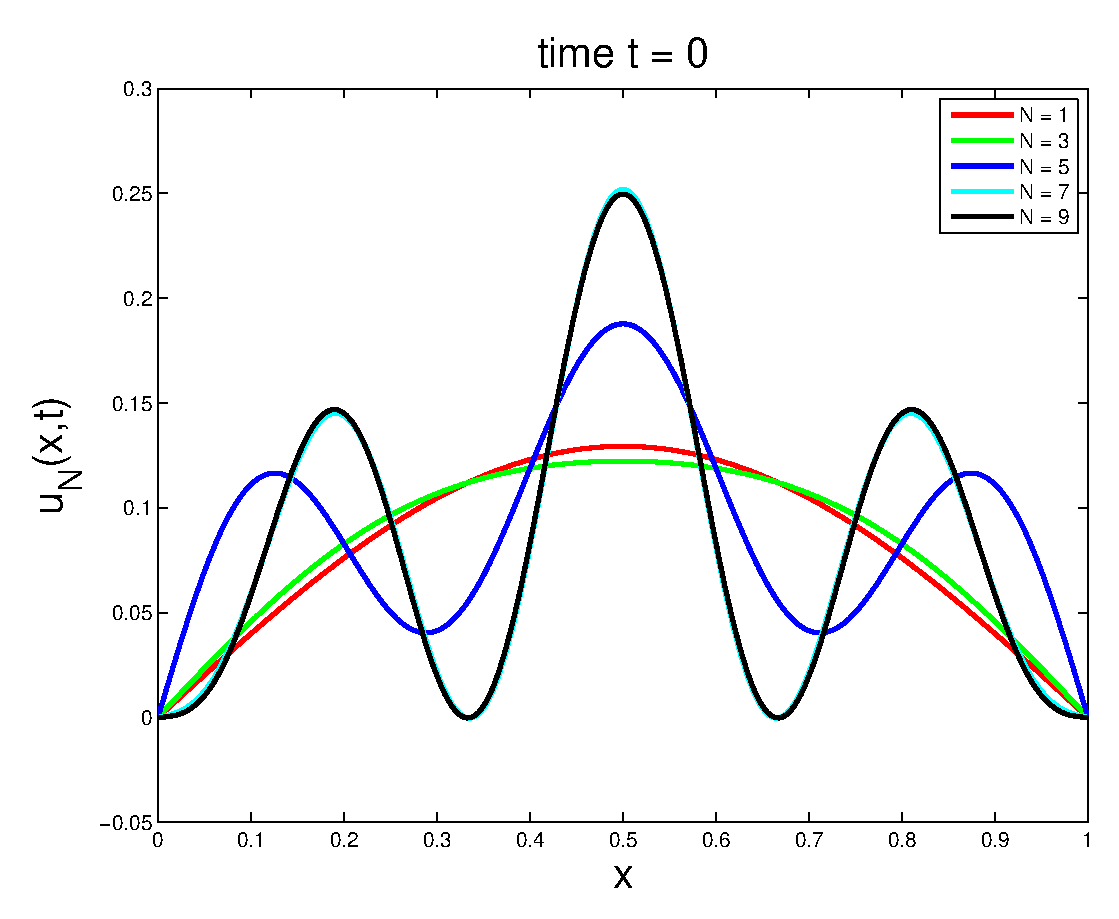
\includegraphics[scale=0.4]{fourth_a}
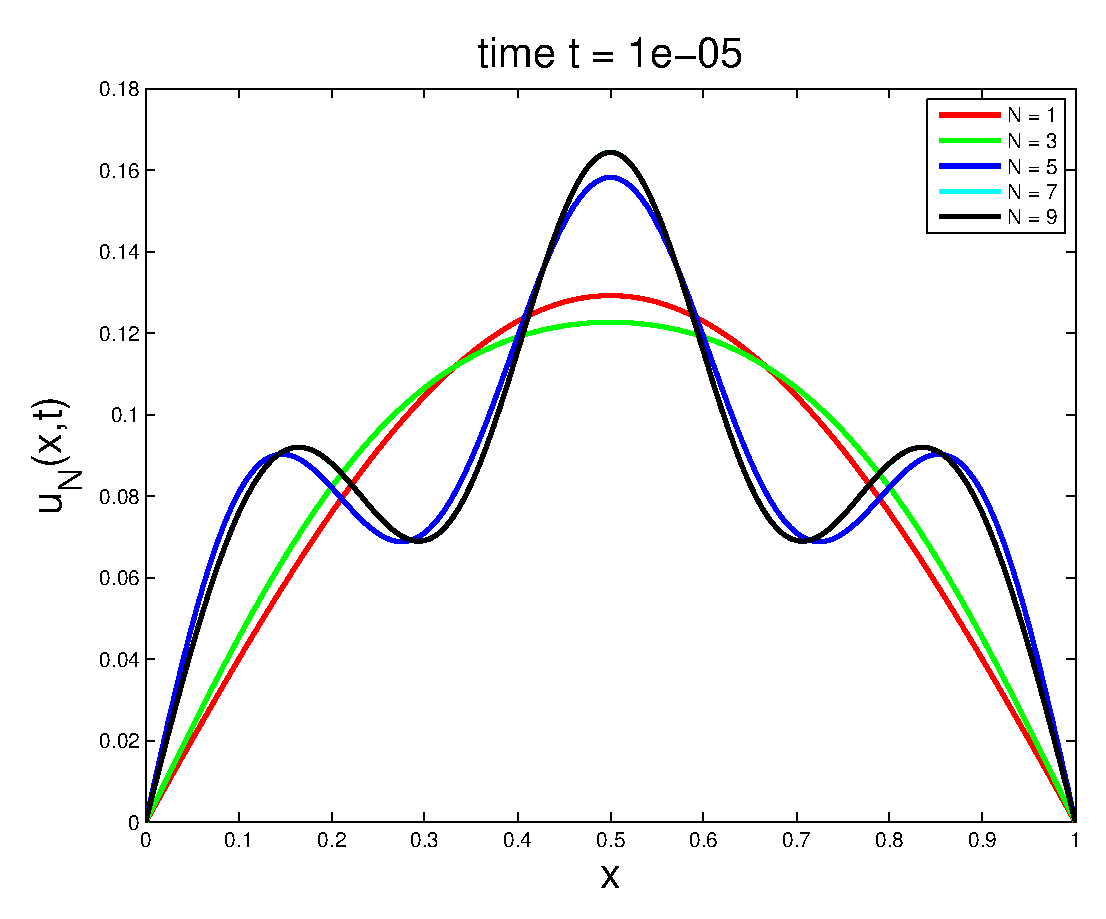
\includegraphics[scale=0.4]{fourth_b}

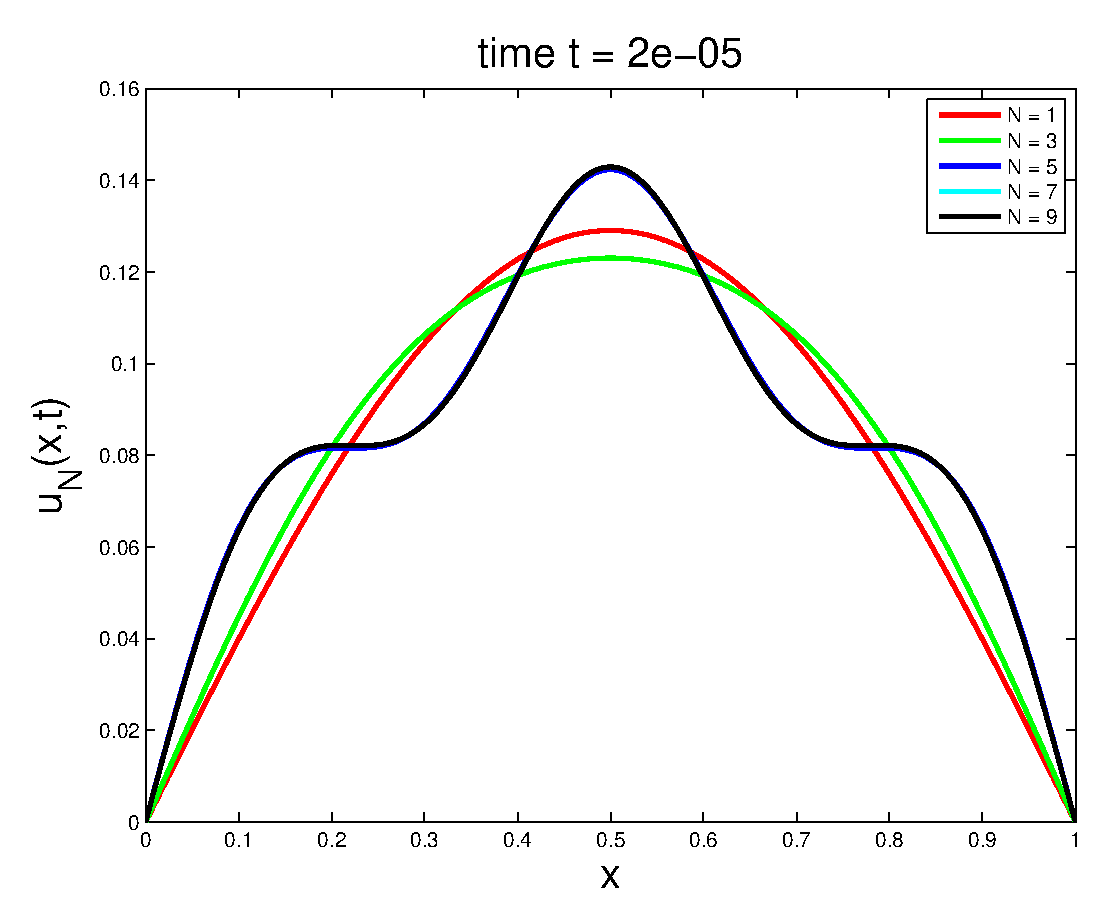
\includegraphics[scale=0.4]{fourth_c}
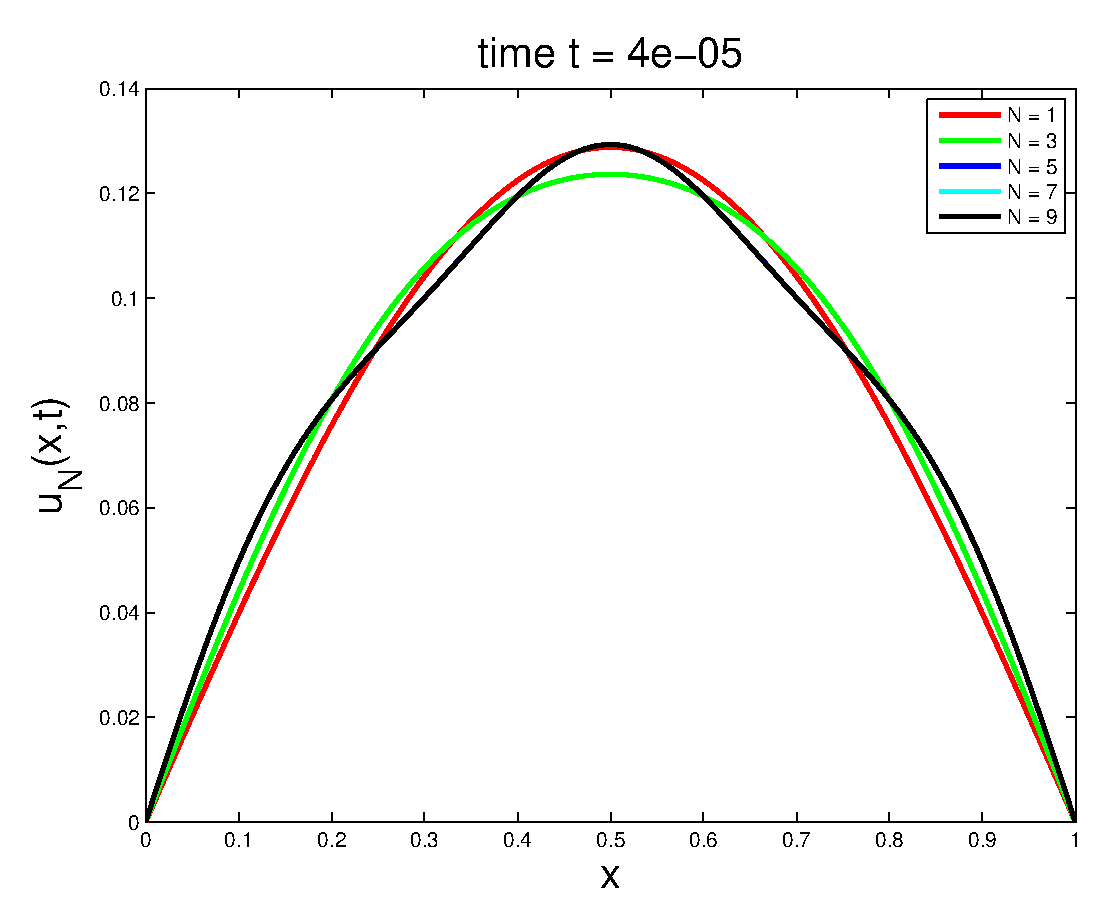
\includegraphics[scale=0.4]{fourth_d}
\end{center}

One can produce these plots with the following code.

\lstinputlisting{HW41.m}

\end{enumerate}
\end{solution}